% Options for packages loaded elsewhere
\PassOptionsToPackage{unicode}{hyperref}
\PassOptionsToPackage{hyphens}{url}
\PassOptionsToPackage{dvipsnames,svgnames,x11names}{xcolor}
%
\documentclass[
  12pt]{article}

\usepackage{amsmath,amssymb}
\usepackage{lmodern}
\usepackage{iftex}
\ifPDFTeX
  \usepackage[T1]{fontenc}
  \usepackage[utf8]{inputenc}
  \usepackage{textcomp} % provide euro and other symbols
\else % if luatex or xetex
  \usepackage{unicode-math}
  \defaultfontfeatures{Scale=MatchLowercase}
  \defaultfontfeatures[\rmfamily]{Ligatures=TeX,Scale=1}
\fi
% Use upquote if available, for straight quotes in verbatim environments
\IfFileExists{upquote.sty}{\usepackage{upquote}}{}
\IfFileExists{microtype.sty}{% use microtype if available
  \usepackage[]{microtype}
  \UseMicrotypeSet[protrusion]{basicmath} % disable protrusion for tt fonts
}{}
\makeatletter
\@ifundefined{KOMAClassName}{% if non-KOMA class
  \IfFileExists{parskip.sty}{%
    \usepackage{parskip}
  }{% else
    \setlength{\parindent}{0pt}
    \setlength{\parskip}{6pt plus 2pt minus 1pt}}
}{% if KOMA class
  \KOMAoptions{parskip=half}}
\makeatother
\usepackage{xcolor}
\setlength{\emergencystretch}{3em} % prevent overfull lines
\setcounter{secnumdepth}{5}
% Make \paragraph and \subparagraph free-standing
\ifx\paragraph\undefined\else
  \let\oldparagraph\paragraph
  \renewcommand{\paragraph}[1]{\oldparagraph{#1}\mbox{}}
\fi
\ifx\subparagraph\undefined\else
  \let\oldsubparagraph\subparagraph
  \renewcommand{\subparagraph}[1]{\oldsubparagraph{#1}\mbox{}}
\fi


\providecommand{\tightlist}{%
  \setlength{\itemsep}{0pt}\setlength{\parskip}{0pt}}\usepackage{longtable,booktabs,array}
\usepackage{calc} % for calculating minipage widths
% Correct order of tables after \paragraph or \subparagraph
\usepackage{etoolbox}
\makeatletter
\patchcmd\longtable{\par}{\if@noskipsec\mbox{}\fi\par}{}{}
\makeatother
% Allow footnotes in longtable head/foot
\IfFileExists{footnotehyper.sty}{\usepackage{footnotehyper}}{\usepackage{footnote}}
\makesavenoteenv{longtable}
\usepackage{graphicx}
\makeatletter
\def\maxwidth{\ifdim\Gin@nat@width>\linewidth\linewidth\else\Gin@nat@width\fi}
\def\maxheight{\ifdim\Gin@nat@height>\textheight\textheight\else\Gin@nat@height\fi}
\makeatother
% Scale images if necessary, so that they will not overflow the page
% margins by default, and it is still possible to overwrite the defaults
% using explicit options in \includegraphics[width, height, ...]{}
\setkeys{Gin}{width=\maxwidth,height=\maxheight,keepaspectratio}
% Set default figure placement to htbp
\makeatletter
\def\fps@figure{htbp}
\makeatother

\addtolength{\oddsidemargin}{-.5in}%
\addtolength{\evensidemargin}{-1in}%
\addtolength{\textwidth}{1in}%
\addtolength{\textheight}{1.7in}%
\addtolength{\topmargin}{-1in}%
\makeatletter
\makeatother
\makeatletter
\makeatother
\makeatletter
\@ifpackageloaded{caption}{}{\usepackage{caption}}
\AtBeginDocument{%
\ifdefined\contentsname
  \renewcommand*\contentsname{Table of contents}
\else
  \newcommand\contentsname{Table of contents}
\fi
\ifdefined\listfigurename
  \renewcommand*\listfigurename{List of Figures}
\else
  \newcommand\listfigurename{List of Figures}
\fi
\ifdefined\listtablename
  \renewcommand*\listtablename{List of Tables}
\else
  \newcommand\listtablename{List of Tables}
\fi
\ifdefined\figurename
  \renewcommand*\figurename{Figure}
\else
  \newcommand\figurename{Figure}
\fi
\ifdefined\tablename
  \renewcommand*\tablename{Table}
\else
  \newcommand\tablename{Table}
\fi
}
\@ifpackageloaded{float}{}{\usepackage{float}}
\floatstyle{ruled}
\@ifundefined{c@chapter}{\newfloat{codelisting}{h}{lop}}{\newfloat{codelisting}{h}{lop}[chapter]}
\floatname{codelisting}{Listing}
\newcommand*\listoflistings{\listof{codelisting}{List of Listings}}
\makeatother
\makeatletter
\@ifpackageloaded{caption}{}{\usepackage{caption}}
\@ifpackageloaded{subcaption}{}{\usepackage{subcaption}}
\makeatother
\makeatletter
\@ifpackageloaded{tcolorbox}{}{\usepackage[many]{tcolorbox}}
\makeatother
\makeatletter
\@ifundefined{shadecolor}{\definecolor{shadecolor}{rgb}{.97, .97, .97}}
\makeatother
\makeatletter
\makeatother
\ifLuaTeX
  \usepackage{selnolig}  % disable illegal ligatures
\fi
\usepackage[]{natbib}
\bibliographystyle{agsm}
\IfFileExists{bookmark.sty}{\usepackage{bookmark}}{\usepackage{hyperref}}
\IfFileExists{xurl.sty}{\usepackage{xurl}}{} % add URL line breaks if available
\urlstyle{same} % disable monospaced font for URLs
\hypersetup{
  pdftitle={Title},
  pdfauthor={Author 1; Author 2},
  pdfkeywords={3 to 6 keywords, that do not appear in the title},
  colorlinks=true,
  linkcolor={blue},
  filecolor={Maroon},
  citecolor={Blue},
  urlcolor={Blue},
  pdfcreator={LaTeX via pandoc}}


\begin{document}


\def\spacingset#1{\renewcommand{\baselinestretch}%
{#1}\small\normalsize} \spacingset{1}


%%%%%%%%%%%%%%%%%%%%%%%%%%%%%%%%%%%%%%%%%%%%%%%%%%%%%%%%%%%%%%%%%%%%%%%%%%%%%%

\date{October 24, 2022}
\title{\bf Title}
\author{
Author 1\thanks{The authors gratefully acknowledge \emph{please remember
to list all relevant funding sources in the unblinded version}.}\\
Department of YYY, University of XXX\\
and\\Author 2\\
Department of ZZZ, University of WWW\\
}
\maketitle

\bigskip
\bigskip
\begin{abstract}
The text of your abstract. 200 or fewer words.
\end{abstract}

\noindent%
{\it Keywords:} 3 to 6 keywords, that do not appear in the title
\vfill

\newpage
\spacingset{1.9} % DON'T change the spacing!
\ifdefined\Shaded\renewenvironment{Shaded}{\begin{tcolorbox}[frame hidden, interior hidden, borderline west={3pt}{0pt}{shadecolor}, boxrule=0pt, enhanced, breakable, sharp corners]}{\end{tcolorbox}}\fi

\hypertarget{sec-intro}{%
\section{Introduction}\label{sec-intro}}

Body of paper. Margins in this document are roughly 0.75 inches all
around, letter size paper.

\begin{figure}

{\centering 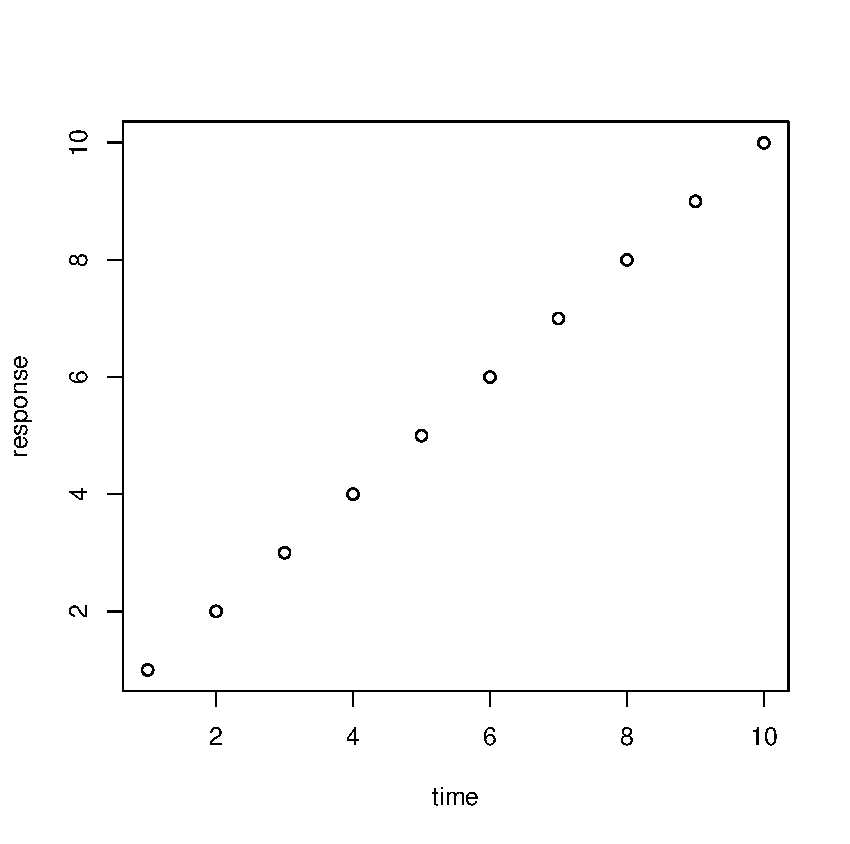
\includegraphics[width=3in,height=\textheight]{fig1.pdf}

}

\caption{\label{fig-first}Consistency comparison in fitting surrogate
model in the tidal power example.}

\end{figure}

\hypertarget{tbl-one}{}
\begin{longtable}[]{@{}lllll@{}}
\caption{\label{tbl-one}D-optimality values for design X under five
different scenarios.}\tabularnewline
\toprule()
one & two & three & four & five \\
\midrule()
\endfirsthead
\toprule()
one & two & three & four & five \\
\midrule()
\endhead
1.23 & 3.45 & 5.00 & 1.21 & 3.41 \\
1.23 & 3.45 & 5.00 & 1.21 & 3.42 \\
1.23 & 3.45 & 5.00 & 1.21 & 3.43 \\
\bottomrule()
\end{longtable}

\begin{itemize}
\tightlist
\item
  Note that figures and tables (such as Figure~\ref{fig-first} and
  Table~\ref{tbl-one}) should appear in the paper, not at the end or in
  separate files.
\item
  In document front matter, you may set the key \texttt{blinded} under a
  \texttt{journal} key to hide the authors and acknowledgements,
  producing the required blinded version.
\item
  Remember that in the blind version, you should not identify authors
  indirectly in the text. That is, don't say ``In Smith et. al.~(2009)
  we showed that \ldots{}''. Instead, say ``Smith et. al.~(2009) showed
  that \ldots{}''.
\item
  These points are only intended to remind you of some requirements.
  Please refer to the instructions for authors at
  \url{http://amstat.tandfonline.com/action/authorSubmission?journalCode=uasa20\&page=instructions\#.VFkk7fnF_0c}
\item
  For more about ASA~style, please see
  \url{http://journals.taylorandfrancis.com/amstat/asa-style-guide/}
\item
  If you have supplementary material (e.g., software, data, technical
  proofs), identify them in the section below. In early stages of the
  submission process, you may be unsure what to include as supplementary
  material. Don't worry---this is something that can be worked out at
  later stages.
\end{itemize}

\hypertarget{sec-meth}{%
\section{Methods}\label{sec-meth}}

Don't take any of these section titles seriously. They're just for
illustration.

\hypertarget{sec-verify}{%
\section{Verifications}\label{sec-verify}}

This section will be just long enough to illustrate what a full page of
text looks like, for margins and spacing.

\addtolength{\textheight}{.5in}%

\citet{Campbell02}, \citet{Schubert13}, \citet{Chi81}

The quick brown fox jumped over the lazy dog. The quick brown fox jumped
over the lazy dog. The quick brown fox jumped over the lazy dog. The
quick brown fox jumped over the lazy dog. \textbf{With this spacing we
have 25 lines per page.} The quick brown fox jumped over the lazy dog.
The quick brown fox jumped over the lazy dog. The quick brown fox jumped
over the lazy dog. The quick brown fox jumped over the lazy dog. The
quick brown fox jumped over the lazy dog.

The quick brown fox jumped over the lazy dog. The quick brown fox jumped
over the lazy dog. The quick brown fox jumped over the lazy dog. The
quick brown fox jumped over the lazy dog. The quick brown fox jumped
over the lazy dog. The quick brown fox jumped over the lazy dog. The
quick brown fox jumped over the lazy dog. The quick brown fox jumped
over the lazy dog. The quick brown fox jumped over the lazy dog. The
quick brown fox jumped over the lazy dog.

The quick brown fox jumped over the lazy dog. The quick brown fox jumped
over the lazy dog. The quick brown fox jumped over the lazy dog. The
quick brown fox jumped over the lazy dog. The quick brown fox jumped
over the lazy dog. The quick brown fox jumped over the lazy dog. The
quick brown fox jumped over the lazy dog. The quick brown fox jumped
over the lazy dog. The quick brown fox jumped over the lazy dog. The
quick brown fox jumped over the lazy dog.

\%new margin nere

The quick brown fox jumped over the lazy dog. The quick brown fox jumped
over the lazy dog. The quick brown fox jumped over the lazy dog. The
quick brown fox jumped over the lazy dog. The quick brown fox jumped
over the lazy dog. The quick brown fox jumped over the lazy dog. The
quick brown fox jumped over the lazy dog. The quick brown fox jumped
over the lazy dog. The quick brown fox jumped over the lazy dog. The
quick brown fox jumped over the lazy dog.

\addtolength{\textheight}{-.5in}%

\addtolength{\textheight}{.2in}%

The quick brown fox jumped over the lazy dog. The quick brown fox jumped
over the lazy dog. The quick brown fox jumped over the lazy dog. The
quick brown fox jumped over the lazy dog. The quick brown fox jumped
over the lazy dog. The quick brown fox jumped over the lazy dog. The
quick brown fox jumped over the lazy dog. The quick brown fox jumped
over the lazy dog. The quick brown fox jumped over the lazy dog. The
quick brown fox jumped over the lazy dog.

The quick brown fox jumped over the lazy dog. The quick brown fox jumped
over the lazy dog. The quick brown fox jumped over the lazy dog. The
quick brown fox jumped over the lazy dog. The quick brown fox jumped
over the lazy dog. The quick brown fox jumped over the lazy dog. The
quick brown fox jumped over the lazy dog. The quick brown fox jumped
over the lazy dog. The quick brown fox jumped over the lazy dog. The
quick brown fox jumped over the lazy dog.

The quick brown fox jumped over the lazy dog. The quick brown fox jumped
over the lazy dog. The quick brown fox jumped over the lazy dog. The
quick brown fox jumped over the lazy dog. The quick brown fox jumped
over the lazy dog. The quick brown fox jumped over the lazy dog. The
quick brown fox jumped over the lazy dog. The quick brown fox jumped
over the lazy dog. The quick brown fox jumped over the lazy dog. The
quick brown fox jumped over the lazy dog.

The quick brown fox jumped over the lazy dog. The quick brown fox jumped
over the lazy dog. The quick brown fox jumped over the lazy dog. The
quick brown fox jumped over the lazy dog. The quick brown fox jumped
over the lazy dog. The quick brown fox jumped over the lazy dog. The
quick brown fox jumped over the lazy dog. The quick brown fox jumped
over the lazy dog. The quick brown fox jumped over the lazy dog. The
quick brown fox jumped over the lazy dog.

The quick brown fox jumped over the lazy dog. The quick brown fox jumped
over the lazy dog. The quick brown fox jumped over the lazy dog. The
quick brown fox jumped over the lazy dog. The quick brown fox jumped
over the lazy dog. The quick brown fox jumped over the lazy dog. The
quick brown fox jumped over the lazy dog. The quick brown fox jumped
over the lazy dog. The quick brown fox jumped over the lazy dog. The
quick brown fox jumped over the lazy dog.

The quick brown fox jumped over the lazy dog. The quick brown fox jumped
over the lazy dog. The quick brown fox jumped over the lazy dog. The
quick brown fox jumped over the lazy dog. The quick brown fox jumped
over the lazy dog. The quick brown fox jumped over the lazy dog. The
quick brown fox jumped over the lazy dog. The quick brown fox jumped
over the lazy dog. The quick brown fox jumped over the lazy dog. The
quick brown fox jumped over the lazy dog.

The quick brown fox jumped over the lazy dog. The quick brown fox jumped
over the lazy dog. The quick brown fox jumped over the lazy dog. The
quick brown fox jumped over the lazy dog.

\addtolength{\textheight}{-.2in}%

\hypertarget{sec-conc}{%
\section{Conclusion}\label{sec-conc}}

\hypertarget{supplementary-material}{}
\bigskip

\begin{center}

{\large\bf SUPPLEMENTARY MATERIAL}

\end{center}

\begin{description}
\item[Title:]
Brief description. (file type)
\item[R-package for MYNEW routine:]
R-package MYNEW containing code to perform the diagnostic methods
described in the article. The package also contains all datasets used as
examples in the article. (GNU zipped tar file)
\item[HIV data set:]
Data set used in the illustration of MYNEW method in
Section\textasciitilde{} 3.2. (.txt file)
\end{description}

\hypertarget{bibtex}{%
\section{BibTeX}\label{bibtex}}

We hope you've chosen to use BibTeX! If you have, please feel free to
use the package natbib with any bibliography style you're comfortable
with. The .bst file agsm has been included here for your convenience.


  \bibliography{bibliography.bib}


\end{document}
